\appendix
\section*{Appendix}

\section{Related Work}
\label{sec:related_work}

\paragraph{Multi-Turn LLM Agents.}
Recent LLM agents extend language models from single-turn text generation to interactive decision making, where the model repeatedly observes an environment, produces an action or tool call, and receives new feedback \citep{yao2022react, yang2024swe, chan2025mle}. These multi-turn agents have been studied in embodied simulators \citep{shridhar2020alfworld}, web navigation \citep{gur2024real, team2025tongyi}, tool use \citep{yao2024tau}, and search-based question answering \citep{jin2025search}. Compared with single-turn tasks, multi-turn agent learning is more challenging because the model must maintain a long interaction history, reason over partially observable states, and recover from its own previous mistakes. An early suboptimal action can change the future observation stream, causing errors to compound across the trajectory \citep{zhang2025agentracer}.

To improve multi-turn agent performance, prior work has mainly explored two training paradigms. The first is multi-turn SFT \citep{teng2024fine, li2025beyond}, which decomposes teacher trajectories into turn-level training examples and trains the model to imitate them. This can improve formatting and local action prediction, but it remains off-policy: the student is optimized on teacher-generated states rather than the histories induced by its own behavior. The second is reinforcement learning with verifiable rewards (RLVR) \citep{shao2024deepseekmath}, where the agent receives reward from the final environment outcome \citep{deepswe2025, wei2025webagent}. While this directly optimizes task success, it typically requires an external verifier or environment-defined reward signal, and the resulting reward is often sparse relative to the long sequence of student-generated turns, making credit assignment difficult~\citep{wang2026openclaw}. These limitations motivate on-policy distillation methods that can provide teacher supervision on student-induced trajectories while avoiding the sparsity of pure outcome-based reward learning.

\paragraph{On-Policy Distillation and Multi-Turn Limitations.}
To mitigate the exposure bias of offline imitation, OPD shifts supervision from teacher-generated trajectories to the student's own generated distribution \citep{agarwal2024policy, lu2025onpolicydistillation}. In OPD, the student first samples trajectories under its current policy, and the teacher then provides token-level feedback on the resulting student-induced states. This aligns training with inference-time behavior and allows the student to learn from states that arise from its own decisions, rather than only from expert demonstrations \citep{zhao2026self, he2026self, hubotter2026reinforcement}.

Despite this advantage, recent analyses have revealed that the token-level logit signal underlying standard OPD is surprisingly brittle. This brittleness is further amplified in multi-turn settings, where local token-level mismatches can compound across turns. First, OPD relies on a narrow token-level overlap between the teacher's and student's plausible next-token distributions \citep{li2026rethinking}. When multiple continuations are semantically valid, dense token-level alignment can over-penalize acceptable alternatives. Second, OPD can reinforce degenerate local patterns when repeated or low-quality prefixes accidentally receive favorable token-level gradients \citep{luo2026demystifying}; in multi-turn agents, this may manifest as repeated thoughts or repeated actions across consecutive turns. Third, multi-turn interaction amplifies distribution shift through compounding errors: student thoughts or actions can push the environment history outside the teacher's effective state distribution, making later teacher supervision less reliable \citep{wang2026tcod, li2025beyond}.

A concurrent line of work, TCOD, addresses this instability by controlling the trajectory depth and gradually expanding the student-controlled horizon through a temporal curriculum \citep{wang2026tcod}. In contrast, \ours{} does not rely on a manually designed curriculum over turn depth. Instead, we delegate the intervention decision to the teacher: for each turn, the teacher determines whether supervision should be skipped, weakly applied, or strongly applied. To further account for compounding errors that may move the student into states where the teacher is less reliable, \ours{} weights the token-level OPD signal by the teacher's predictive confidence. Thus, rather than deciding \emph{how long} to apply OPD, \ours{} decides \emph{where} OPD should be applied and how strongly it should be trusted.

\section{Proofs for Selective Weighting Analysis}
\label{sec:appendix_theory}

\begin{proof}[Proof of Proposition~\ref{prop:relative_suppression}]
For a fixed batch, the noisy component of the normalized selective objective is
\[
    Z\sum_{t=0}^{T-1}s_t\xi_t
    =
    \sum_{t=0}^{T-1}\widetilde{s}_t\xi_t,
\]
where $\widetilde{s}_t=Zs_t$.
%
The variance contribution of turn $t$ is
\[
    \mathrm{Var}[\widetilde{s}_t\xi_t]
    =
    \widetilde{s}_t^2\mathrm{Var}[\xi_t]
    \leq
    \widetilde{s}_t^2\sigma_t^2,
\]
which proves \eqref{eq:noise_bound}.
%
For any two turns $p$ and $q$, the shared normalization factor cancels:
\[
    \frac{\widetilde{s}_p^2}{\widetilde{s}_q^2}
    =
    \frac{Z^2s_p^2}{Z^2s_q^2}
    =
    \frac{s_p^2}{s_q^2}.
\]
%
Therefore, if $s_p\leq\gamma s_q$ for $\gamma<1$, then $\widetilde{s}_p^2/\widetilde{s}_q^2\leq\gamma^2$.
\end{proof}

\begin{proof}[Proof of Proposition~\ref{prop:oracle_approx}]
By the triangle inequality and the bounded-loss assumption,
\[
\begin{aligned}
\left|
\sum_{t=0}^{T-1}
(s_t-m_t^\star)\ell_t(\theta)
\right|
&\leq
\sum_{t=0}^{T-1}
|s_t-m_t^\star|\,|\ell_t(\theta)| \\
&\leq
B\sum_{t=0}^{T-1}
|s_t-m_t^\star|.
\end{aligned}
\]
%
This proves \eqref{eq:oracle_bound}.
\end{proof}

\section{Implementation Details}
\label{sec:implementation_details}


We implement \ours{} and all baselines on top of the \texttt{verl} fully-asynchronous pipeline, using a decoupled rollouter--trainer architecture with a staleness-bounded queue. We set \texttt{trigger\_parameter\_sync\_step} to $4$ and \texttt{staleness\_threshold} to $0.5$. We use AdamW with a learning rate $10^{-6}$, weight decay $0.1$, response length $4096$, rollout number $n=1$, global batch size 64, and epoch number 1. 

The maximum number of turns is $30$ for ALFWorld and ScienceWorld and $16$ for SearchQA.
%
The maximum generation length is $4096$ tokens per turn.
%
We use student temperature $0.4$, teacher temperature $0.0$, top-$p=1.0$, and top-$k=-1$ as the default setup.
%
All evaluations use the ReAct prompt format with full chat history, no sliding window, thinking mode disabled, and \texttt{</action>} as the stop string.
%
For SearchQA, the agent is allowed at most $8$ search calls per episode and retrieves the top $3$ documents from a Wikipedia-2018 index using dense E5 retrieval with FAISS-Flat.
%
We evaluate on the standard ALFWorld valid-seen and valid-unseen splits, the ScienceWorld test set with $30$ task types and $5$ variations per task, and capped SearchQA splits with up to $500$ questions per split except Bamboogle, which contains $125$ questions.


For agentic OPD baselines, we keep the OPD backbone fixed and modify only the per-token or per-turn weighting scheme. TCOD-F2B truncates each rollout after
\begin{equation}
    k(n) = \min\left(k_{\mathrm{start}} + \frac{n}{\eta}, T\right)
\end{equation}
assistant turns. We set $k_{\mathrm{start}}=1$ and $\eta=1$. The maximum horizon is $T=30$ for ALFWorld and ScienceWorld, and $T=16$ for SearchQA, so the curriculum reaches the cap within one epoch. Entropy-Aware OPD scales the per-token weight by
\begin{equation}
    1 + \alpha_e \cdot \mathbf{1}
    \left[
    H_{\phi}(\cdot \mid h_t,a_{t,<j}) > \tau_e
    \right],
\end{equation}
where $H_{\phi}$ is estimated from the cached top-$K$ teacher distribution. We use $\tau_e=0.8$ and $\alpha_e=1.0$.

For \ours{}, the selective weight is defined as
\begin{equation}
    s_t = i_t \cdot c_t.
\end{equation}
The default per-turn intervention weight $i_t \in \{0,0.5,1\}$ ($\alpha=0.5$) is obtained from one short teacher query per assistant turn, using maximum generation length $1028$ and default temperature $0.0$. If the teacher output is unparseable, we conservatively fall back to $i_t=1$. We also retain the deterministic-failure short circuit: if the student turn is empty, unparseable, or violates the required action schema, we directly set $i_t=1$ without relying on the teacher intervention query.

We use the training split of each benchmark for training. For SearchQA \citep{jin2025search}, we randomly sample 10K examples from the training split as the training subset.

\paragraph{Evaluation Metrics.}
We use benchmark-specific metrics following the standard evaluation protocols.
%
For ALFWorld, we report success rate (SR) on the valid-seen and valid-unseen splits, where an episode is counted as successful if the environment returns \texttt{info["won"] = True} within the turn budget.
%
For ScienceWorld, we report both SR and mean score.
%
SR counts episodes whose cumulative score reaches $100$, while mean score averages the environment-provided cumulative reward over episodes.
%
Since ScienceWorld provides partial credit and small models rarely solve tasks end-to-end, mean score is a more sensitive measure of partial progress and catastrophic failures.
%
For SearchQA, we report exact match (EM), where the final answer is counted as correct if its normalized string matches any reference answer.
%
We follow the SearchR1 normalization protocol, which lowercases text, removes punctuation and articles, and collapses whitespace.
%
For SearchQA, we report EM on each evaluation split and macro-average across NQ, TriviaQA, PopQA, HotpotQA, 2WikiMultiHopQA, Musique, and Bamboogle.
%
We also report average number of turns for ALFWorld and ScienceWorld, and average search/turn statistics for SearchQA as auxiliary efficiency metrics.


\section{Supplementary Results}
\label{sec:supplementary_results}


\subsection{Intervention Analysis}
\label{sec:appendix_intervention_analysis}

\begin{figure*}[t]
    \centering
    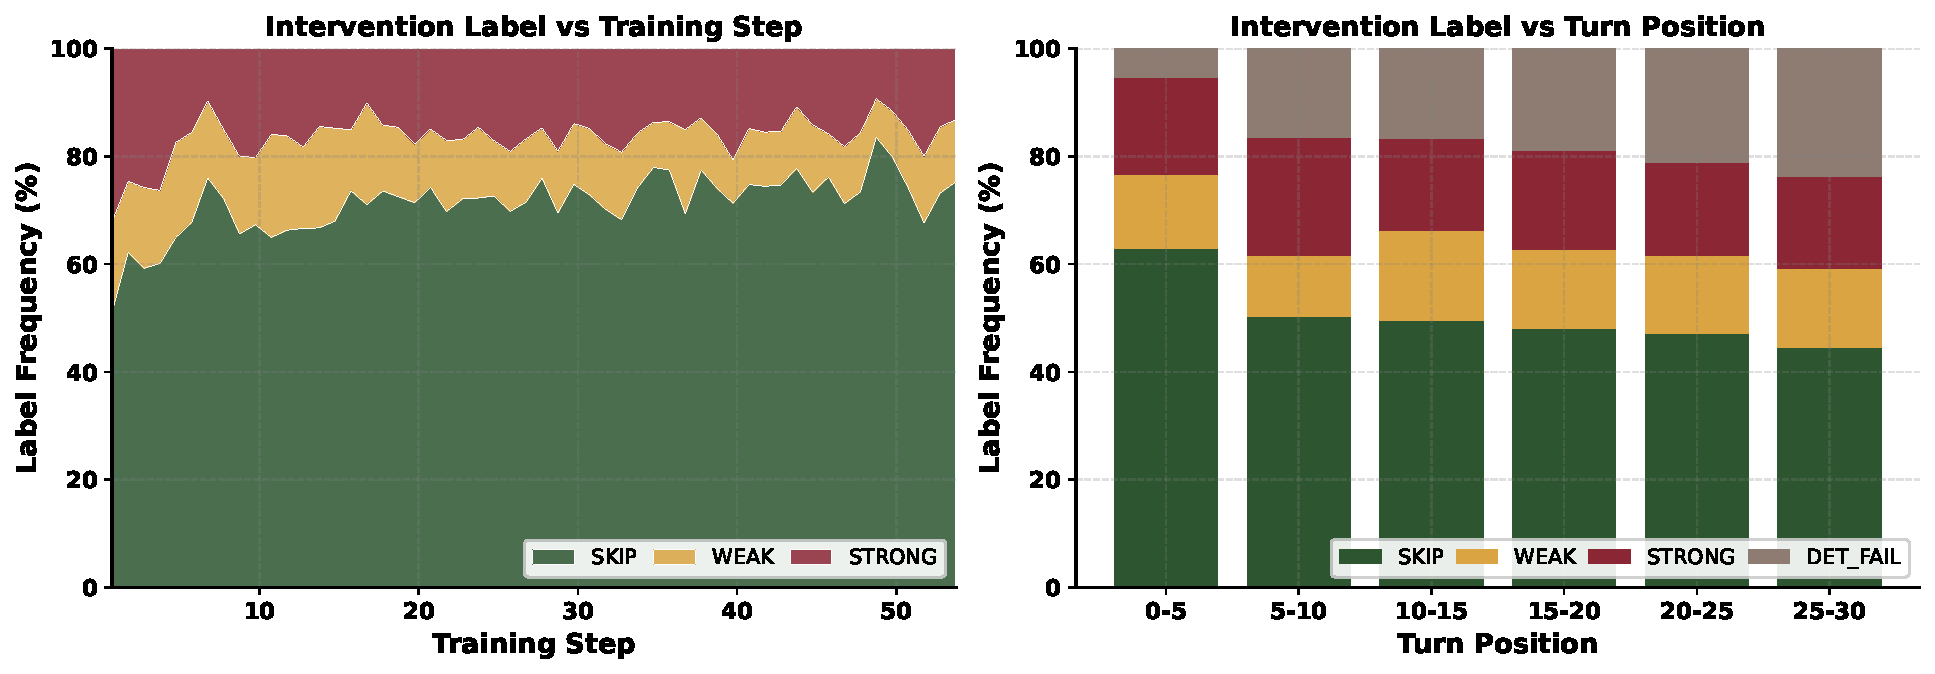
\includegraphics[width=0.9\textwidth]{figure/alfworld_slopd_intervention.pdf}
    \caption{Intervention label distribution of \ours{} on ALFWorld. Left: label frequency across training steps. Right: label frequency across turn positions. \textsc{Det-Fail} denotes deterministic failures detected before teacher intervention, such as malformed actions, failed tool calls, missing executable actions, or environment-reported execution failures.}
    \label{fig:intervention_analysis}
\end{figure*}

\figref{fig:intervention_analysis} analyzes the intervention labels produced by \ours{} across training steps and turn positions.
%
In addition to the teacher-assigned labels \textsc{Skip}, \textsc{Weak}, and \textsc{Strong}, we report \textsc{Det-Fail}, which corresponds to the deterministic-failure short circuit described in \secref{sec:method_intervention}.
%
These are turns where the environment or action parser provides clear negative feedback, such as malformed actions, failed tool calls, missing executable actions, or execution failures.
%
Such turns are directly assigned full intervention without requiring additional teacher judgment.

As training progresses, the proportion of \textsc{Skip} labels generally increases, while \textsc{Weak} and \textsc{Strong} labels decrease.
%
This suggests that the student produces more acceptable actions over time, and the intervention mechanism correspondingly reduces unnecessary teacher supervision.
%
The turn-position analysis shows that \textsc{Skip} remains the dominant label across the trajectory, but gradually decreases as the turn index increases.
%
Meanwhile, \textsc{Det-Fail} becomes more frequent in later turns, indicating that response quality becomes harder to maintain as the interaction horizon grows.
%
This aligns with the compounding-error challenge in multi-turn agents and shows that \ours{} does not simply downweight late supervision uniformly; instead, it distinguishes between turns that can be skipped, turns requiring semantic intervention, and turns with clear execution failures.

\subsection{Ablation Studies}
\label{sec:appendix_ablation}

\begin{table*}[t]
\centering
\caption{Ablation study on ALFWorld. We incrementally evaluate the contribution of turn-level intervention, teacher confidence weighting, and vanilla-scale normalization. Best SR within each student--teacher setup is in \textbf{bold}, and the second-best SR is \underline{underlined}.}
\label{tab:ablation_alfworld}
\resizebox{0.9\textwidth}{!}{%
\begin{tabular}{lllcccc}
\toprule
\textbf{Student Model} & \textbf{Teacher Model} & \textbf{Method}
& \textbf{Seen SR} & \textbf{Seen Turns}
& \textbf{Unseen SR} & \textbf{Unseen Turns} \\
\midrule
\multicolumn{7}{c}{\textit{Student: Qwen3-0.6B, Teacher: Qwen3-8B}} \\
\midrule
\multirow{3}{*}{Qwen3-0.6B} & \multirow{3}{*}{Qwen3-8B}
& Intervention-only & \underline{57.86} & 17.80 & \textbf{62.69} & 18.49 \\
& & \ours{}-NoNorm & 55.71 & 19.19 & 55.22 & 20.50 \\
& & \ours{} & \textbf{57.86} & 18.46 & \underline{61.94} & 18.89 \\
\midrule
\multicolumn{7}{c}{\textit{Student: Qwen3-1.7B, Teacher: Qwen3-8B}} \\
\midrule
\multirow{3}{*}{Qwen3-1.7B} & \multirow{3}{*}{Qwen3-8B}
& Intervention-only & 59.29 & 18.39 & \underline{66.42} & 17.68 \\
& & \ours{}-NoNorm & \textbf{66.43} & 17.15 & 64.93 & 18.51 \\
& & \ours{} & \underline{64.29} & 18.14 & \textbf{70.15} & 17.86 \\
\midrule
\multicolumn{7}{c}{\textit{Student: Qwen3-0.6B, Teacher: Qwen3-32B}} \\
\midrule
\multirow{3}{*}{Qwen3-0.6B} & \multirow{3}{*}{Qwen3-32B}
& Intervention-only & 53.86 & 19.21 & 67.16 & 19.40 \\
& & \ours{}-NoNorm & \textbf{57.86} & 19.61 & \underline{69.40} & 18.10 \\
& & \ours{} & \underline{54.29} & 19.85 & \textbf{70.90} & 17.98 \\
\midrule
\multicolumn{7}{c}{\textit{Student: Qwen3-1.7B, Teacher: Qwen3-32B}} \\
\midrule
\multirow{3}{*}{Qwen3-1.7B} & \multirow{3}{*}{Qwen3-32B}
& Intervention-only & \underline{62.14} & 18.29 & \textbf{79.10} & 16.12 \\
& & \ours{}-NoNorm & 61.43 & 18.39 & 73.13 & 17.14 \\
& & \ours{} & \textbf{62.82} & 18.75 & \underline{73.88} & 17.57 \\
\bottomrule
\end{tabular}%
}
\end{table*}

We conduct ablation studies on ALFWorld to isolate the contribution of each component in \ours{}.
%
\tabref{tab:ablation_alfworld} presents an incremental comparison among three variants: \textit{Intervention-only}, which uses only the turn-level intervention weight $i_t$; \ours{}-NoNorm, which further incorporates teacher confidence weighting $c_t$; and the full \ours{} objective, which additionally applies vanilla-scale normalization.
%
Intervention-only already performs strongly across settings, reaching $62.69$ unseen SR for Qwen3-0.6B distilled from Qwen3-8B and $79.10$ unseen SR for Qwen3-1.7B distilled from Qwen3-32B.
%
This suggests that turn-level intervention labels can identify useful correction points without requiring a task-level verifier.

Adding confidence weighting gives \ours{}-NoNorm, which improves some settings but can also reduce unseen generalization when the selective weights shrink the effective training signal.
%
Vanilla-scale normalization addresses this issue by preserving the overall loss scale while retaining the relative turn-level weights.
%
For example, with Qwen3-1.7B distilled from Qwen3-8B, normalization improves unseen SR from $64.93$ under \ours{}-NoNorm to $70.15$ under the full \ours{} objective; with Qwen3-0.6B distilled from Qwen3-32B, it improves unseen SR from $69.40$ to $70.90$.
%
Overall, the results show that intervention weighting, teacher confidence, and loss-scale normalization play complementary roles in selective multi-turn OPD.

\subsection{Case Study: Turn-Level Intervention Examples}
\label{sec:case_study}

To qualitatively examine how \ours{} allocates teacher supervision, we present representative ALFWorld cases for different intervention outcomes.
%
These examples illustrate that the intervention mechanism does not simply supervise every student response uniformly.
%
Instead, it distinguishes between acceptable actions, mildly suboptimal actions, clearly harmful actions, and deterministic execution failures.

\paragraph{Skip: acceptable student behavior.}
When the student response is reasonable under the current observation, \ours{} assigns \textsc{Skip} and suppresses the OPD loss for that turn.
%
For example, in a \texttt{pick\_two\_obj\_and\_place} task, the student observes the following environment state:
%
\begin{quote}
\small
\texttt{You arrive at coffeetable 1. On the coffeetable 1, you see a box 2, a creditcard 2, a creditcard 1, a houseplant 1, a plate 2, a plate 1, a statue 1, and a wateringcan 1.}
\end{quote}
%
The student responds:
%
\begin{quote}
\small
\texttt{Thought: I need to find two vases and place them on the coffeetable.}\\
\texttt{Action: look}
\end{quote}
%
The parsed action is \texttt{look}, and the teacher assigns \textsc{Skip} with intervention weight $i_t=0$.
%
Although the action does not immediately complete the task, it is a valid exploratory step under the current observation.
%
In another \texttt{pick\_clean\_then\_place\_in\_recep} task, the student similarly takes an exploratory action:
%
\begin{quote}
\small
\texttt{Thought: I need to examine the cabinet to find a knife.}\\
\texttt{Action: examine cabinet 1}
\end{quote}
%
The environment returns that the cabinet contains nothing, but the action itself is executable and plausible, so the teacher again assigns \textsc{Skip}.
%
These cases show that \ours{} avoids unnecessary token-level correction when the student is making plausible progress.

\paragraph{Weak: executable but suboptimal behavior.}
When the student action is valid but potentially inefficient or only partially aligned with the task, \ours{} assigns \textsc{Weak}.
%
For instance, in a \texttt{pick\_clean\_then\_place\_in\_recep} task, the student sees the same coffeetable observation and produces:
%
\begin{quote}
\small
\texttt{Thought: I need to find a clean kettle in the cabinet.}\\
\texttt{Action: examine cabinet 1}
\end{quote}
%
The action \texttt{examine cabinet 1} is executable and may still provide useful information, but it is not clearly the best next step for the task.
%
The teacher therefore assigns \textsc{Weak} with intervention weight $i_t=\alpha$.
%
As another example, in a \texttt{pick\_and\_place\_simple} task, the student reasons:
%
\begin{quote}
\small
\texttt{Thought: The cloth is not on the countertop. I'll check the cabinets to find a cloth.}\\
\texttt{Action: go to cabinet 1}
\end{quote}
%
The environment accepts the action and moves the agent to the closed cabinet, but the decision remains uncertain rather than clearly optimal.
%
The teacher again assigns \textsc{Weak}.
%
These examples demonstrate that \ours{} can provide partial supervision for ambiguous turns rather than forcing a binary choice between full imitation and no correction.

\paragraph{Strong: clearly harmful or inconsistent behavior.}
When the student response is clearly inconsistent with the task state or likely to push the trajectory in an unhelpful direction, \ours{} assigns \textsc{Strong}.
%
For example, in a \texttt{pick\_cool\_then\_place\_in\_recep} task, the student states that it should cool a plate in the fridge, but then navigates to a cabinet:
%
\begin{quote}
\small
\texttt{Thought: I need to find a plate and cool it in the fridge before putting it in the cabinet.}\\
\texttt{Action: go to cabinet 1}
\end{quote}
%
This response is internally inconsistent with the required cooling procedure, because moving to a cabinet does not help complete the cooling step.
%
The teacher assigns \textsc{Strong} with intervention weight $i_t=1$.
%
A related failure occurs when the student repeats the same high-level intent but selects another cabinet-navigation action:
%
\begin{quote}
\small
\texttt{Thought: I need to find a plate and cool it in the fridge before putting it in the cabinet.}\\
\texttt{Action: go to cabinet 10}
\end{quote}
%
Although the action is executable, it is unlikely to make progress toward cooling the object and may cause the trajectory to drift further from a successful plan.
%
These cases show that strong intervention is used when the current turn requires clear correction.

\paragraph{Deterministic failure: environment-detected execution error.}
In addition to teacher-judged intervention, \ours{} directly assigns full intervention when the environment or parser detects a deterministic failure.
%
For example, in a \texttt{pick\_and\_place\_simple} task, the student attempts:
%
\begin{quote}
\small
\texttt{Thought: I need to place the book on the sofa. I'll put the book on the sofa now.}\\
\texttt{Action: put book 1 in/on sofa 1}
\end{quote}
%
The parsed action is \texttt{put book 1 in/on sofa 1}, but the environment returns:
%
\begin{quote}
\small
\texttt{Nothing happens.}
\end{quote}
%
Similarly, in another episode, the student outputs:
%
\begin{quote}
\small
\texttt{Thought: I need to put the laptop in the safe. I'll put the laptop in the safe now.}\\
\texttt{Action: put laptop 1 in/on safe 1}
\end{quote}
%
Again, the environment returns \texttt{Nothing happens}, indicating that the action failed to produce a valid state transition.
%
In these cases, \ours{} bypasses semantic teacher judgment and directly applies full intervention with $i_t=1$.
%
This deterministic-failure pathway provides a high-precision correction signal for malformed, invalid, or ineffective executable actions.

\paragraph{Discussion.}
Overall, these case studies support the motivation for selective multi-turn OPD.
%
Different student turns require different levels of teacher supervision: some should be left unchanged, some benefit from weak guidance, and others require strong correction.
%
By using environment feedback together with teacher judgment, \ours{} allocates supervision at the turn level and avoids applying dense token-level OPD uniformly across the entire trajectory.
%
This behavior is especially important in multi-turn environments, where over-correcting acceptable exploration can reduce behavioral diversity, while failing to intervene on invalid or harmful actions can cause errors to compound in later turns.



\begin{table*}[t]
\centering
\caption{Main results on ScienceWorld. We report success rate (SR), mean task score, and average number of turns. Best SR among distillation methods for each student--teacher setup is in \textbf{bold}, and the second-best SR is \underline{underlined}.}
\label{tab:main_results_scienceworld}
% \resizebox{0.9\textwidth}{!}{%
\begin{tabular}{lllccc}
\toprule
\textbf{Student Model} & \textbf{Teacher Model} & \textbf{Method}
& \textbf{SR} & \textbf{Mean Score} & \textbf{Turns} \\
\midrule
\multicolumn{6}{c}{\textit{Reference Models (Base Inference)}} \\
\midrule
Qwen3-0.6B & -- & Base & 3.36 & -43.51 & 21.38 \\
Qwen3-1.7B & -- & Base & 3.36 & -24.00 & 21.38 \\
-- & Qwen3-8B & Base & 10.74 & -16.09 & 21.67 \\
-- & Qwen3-32B & Base & 15.44 & -17.92 & 18.67 \\
\midrule
\multicolumn{6}{c}{\textit{Student: Qwen3-0.6B, Teacher: Qwen3-8B}} \\
\midrule
\multirow{5}{*}{Qwen3-0.6B} & \multirow{5}{*}{Qwen3-8B} & SFT & 2.01 & -31.84 & 23.94 \\
 & & OPD & 2.01 & -12.88 & 23.94 \\
 & & Entropy-Aware OPD & \textbf{3.36} & -11.52 & 23.44 \\
 & & TCOD-F2B & \underline{3.03} & -2.07 & 24.88 \\
 & & \ours{} & 2.01 & \textbf{+3.89} & 26.94 \\
\midrule
\multicolumn{6}{c}{\textit{Student: Qwen3-1.7B, Teacher: Qwen3-8B}} \\
\midrule
\multirow{5}{*}{Qwen3-1.7B} & \multirow{5}{*}{Qwen3-8B} & SFT & 2.01 & -17.56 & 23.28 \\
 & & OPD & 4.70 & -2.78 & 25.12 \\
 & & Entropy-Aware OPD & 3.36 & -3.13 & 25.91 \\
 & & TCOD-F2B & 4.70 & -9.68 & 24.06 \\
 & & \ours{} & \textbf{6.71} & \textbf{+0.24} & 25.30 \\
\midrule
\multicolumn{6}{c}{\textit{Student: Qwen3-0.6B, Teacher: Qwen3-32B}} \\
\midrule
\multirow{5}{*}{Qwen3-0.6B} & \multirow{5}{*}{Qwen3-32B} & SFT & 2.01 & -34.59 & 18.10 \\
 & & OPD & 3.36 & -28.46 & 20.79 \\
 & & Entropy-Aware OPD & \textbf{6.04} & \textbf{-26.10} & 20.00 \\
 & & TCOD-F2B & 2.68 & -33.42 & 23.20 \\
 & & \ours{} & \textbf{6.04} & \textbf{-26.10} & 20.00 \\
\midrule
\multicolumn{6}{c}{\textit{Student: Qwen3-1.7B, Teacher: Qwen3-32B}} \\
\midrule
\multirow{5}{*}{Qwen3-1.7B} & \multirow{5}{*}{Qwen3-32B} & SFT & 2.01 & -15.61 & 23.23 \\
 & & OPD & 4.03 & -29.89 & 19.64 \\
 & & Entropy-Aware OPD & 3.36 & -14.99 & 23.59 \\
 & & TCOD-F2B & \underline{6.04} & \textbf{-14.89} & 22.02 \\
 & & \ours{} & \textbf{7.38} & -16.01 & 20.91 \\
\bottomrule
\end{tabular}%
% }
\end{table*}


\begin{table*}[t]
\centering
\caption{Main results on SearchQA. We report exact match (EM) across seven question-answering datasets and their average. Best average among distillation methods for each student--teacher setup is in \textbf{bold}, and the second-best average is \underline{underlined}.}
\label{tab:main_results_searchqa}
\resizebox{\textwidth}{!}{%
\begin{tabular}{lllcccccccc}
\toprule
\textbf{Student Model} & \textbf{Teacher Model} & \textbf{Method}
& \textbf{NQ} & \textbf{TriviaQA} & \textbf{PopQA} & \textbf{HotpotQA}
& \textbf{2WikiMQA} & \textbf{Musique} & \textbf{Bamboogle} & \textbf{Avg.} \\
\midrule
\multicolumn{11}{c}{\textit{Reference Models (Base Inference)}} \\
\midrule
Qwen3-0.6B & -- & Base & 5.60 & 15.40 & 0.40 & 6.00 & 8.40 & 1.20 & 3.20 & 5.74 \\
Qwen3-1.7B & -- & Base & 24.20 & 36.40 & 5.20 & 19.00 & 14.20 & 10.80 & 18.40 & 18.31 \\
-- & Qwen3-8B & Base & 34.60 & 53.00 & 14.00 & 38.20 & 37.40 & 28.80 & 45.60 & 35.94 \\
-- & Qwen3-14B & Base & 35.00 & 55.80 & 15.60 & 41.20 & 43.00 & 30.00 & 49.60 & 38.60 \\
\midrule
\multicolumn{11}{c}{\textit{Student: Qwen3-0.6B, Teacher: Qwen3-8B}} \\
\midrule
\multirow{5}{*}{Qwen3-0.6B} & \multirow{5}{*}{Qwen3-8B} & SFT & 14.40 & 23.60 & 5.80 & 13.20 & 11.69 & 2.23 & 6.40 & 11.05 \\
 & & OPD & 25.00 & 41.40 & 17.80 & 28.20 & 24.80 & 17.00 & 24.00 & 25.46 \\
 & & Entropy-Aware OPD & \textbf{25.60} & 40.00 & \textbf{18.80} & 28.80 & \textbf{25.60} & \underline{17.40} & \textbf{24.40} & \textbf{25.80} \\
 & & TCOD-F2B & \underline{25.40} & 41.00 & 15.60 & \underline{29.00} & 24.60 & 16.80 & 23.20 & 25.09 \\
 & & \ours{} & 25.20 & \textbf{41.60} & \underline{18.40} & \textbf{29.80} & 23.20 & 15.00 & \underline{24.00} & \underline{25.31} \\
\midrule
\multicolumn{11}{c}{\textit{Student: Qwen3-1.7B, Teacher: Qwen3-8B}} \\
\midrule
\multirow{5}{*}{Qwen3-1.7B} & \multirow{5}{*}{Qwen3-8B} & SFT & 27.40 & 39.60 & 11.60 & 21.20 & 8.80 & 12.00 & 20.00 & 20.09 \\
 & & OPD & 30.60 & 47.20 & 12.40 & 33.20 & 29.60 & \textbf{24.80} & 32.80 & 30.09 \\
 & & Entropy-Aware OPD & 29.40 & \underline{48.20} & 12.60 & 33.20 & \underline{30.20} & 23.80 & \textbf{36.80} & \underline{30.60} \\
 & & TCOD-F2B & \textbf{31.20} & 47.60 & 12.40 & \textbf{33.80} & 28.60 & 24.00 & \underline{36.00} & 30.51 \\
 & & \ours{} & \underline{30.00} & \textbf{48.40} & \textbf{12.80} & 33.20 & \textbf{30.40} & \underline{24.60} & \underline{36.00} & \textbf{30.77} \\
\bottomrule
\end{tabular}%
}
\end{table*}


\section{Prompt Templates}
\label{sec:appendix_prompts}


We use task-specific ReAct-style prompts for each benchmark. All prompts enforce a fixed output protocol so that the executable action can be reliably parsed and sent to the environment. We present the prompt details in \tabref{tab:prompt_alfworld}, \tabref{tab:prompt_scienceworld} and \tabref{tab:prompt_searchqa}. 


In addition to the task-specific agent prompts, \ours{} uses a separate intervention prompt to obtain turn-level teacher judgments.
%
Given the task goal, current environment state, admissible actions, and the student's candidate response, the teacher assigns one label from \{\textsc{Skip}, \textsc{Weak}, \textsc{Strong}\}.
%
The prompt is shown in \tabref{tab:prompt_intervention}.

\begin{table*}[t]
\centering
\caption{Prompt template for ALFWorld. We use a demonstration before the user turn.}
\label{tab:prompt_alfworld}
\resizebox{0.95\textwidth}{!}{%
\begin{tabular}{lp{0.78\textwidth}}
\toprule
\textbf{Field} & \textbf{Prompt Content} \\
\midrule
System prompt &
\begin{minipage}[t]{0.78\textwidth}
\ttfamily
You are an embodied agent solving a household task in a text-based simulator (AlfWorld). You receive an Observation describing what you can see and a list of Admissible commands you may execute. On every turn you must reply with exactly two lines: Thought: <one short sentence of reasoning> Action: <one command, copied verbatim from the Admissible list when possible> Plan briefly, then issue the next action. Only the line beginning with 'Action:' is used to step the environment. Do not add any other text after the Action line.
\end{minipage}
\\
\midrule
One-shot demonstration &
\begin{minipage}[t]{0.78\textwidth}
\ttfamily
An one-shot demonstration.
\end{minipage}
\\
\midrule
User turn &
\begin{minipage}[t]{0.78\textwidth}
\ttfamily
Task: \{task\_goal\}\\
Observation: \{scene\_description\}\\
Admissible: cmd1; cmd2; ...; cmd30 (+N more)
\end{minipage}
\\
\midrule
Assistant turn &
\begin{minipage}[t]{0.78\textwidth}
\ttfamily
Thought: <reasoning>\\
Action: <command>
\end{minipage}
\\
\bottomrule
\end{tabular}%
}
\end{table*}

\begin{table*}[t]
\centering
\caption{Prompt template for ScienceWorld. We use a single generic one-shot ReAct trajectory.}
\label{tab:prompt_scienceworld}
\resizebox{0.95\textwidth}{!}{%
\begin{tabular}{lp{0.78\textwidth}}
\toprule
\textbf{Field} & \textbf{Prompt Content} \\
\midrule
System prompt &
\begin{minipage}[t]{0.78\textwidth}
\ttfamily
You are an embodied agent solving a science task in the ScienceWorld text-based simulator. You receive an Observation describing what you can see and an Inventory listing what you carry. On every turn you must reply with exactly two lines: Thought: <one short sentence of reasoning> Action: <one valid action> Plan briefly, then issue the next action. Only the line beginning with 'Action:' is used to step the environment.
\end{minipage}
\\
\midrule
One-shot demonstration &
\begin{minipage}[t]{0.78\textwidth}
\ttfamily
A single generic ReAct trajectory.
\end{minipage}
\\
\midrule
User turn &
\begin{minipage}[t]{0.78\textwidth}
\ttfamily
Task: \{task\_description\}\\
Observation: \{observation\}\\
Inventory: \{inventory or "(empty)"\}
\end{minipage}
\\
\midrule
Assistant turn &
\begin{minipage}[t]{0.78\textwidth}
\ttfamily
Thought: <reasoning>\\
Action: <valid action>
\end{minipage}
\\
\bottomrule
\end{tabular}%
}
\end{table*}

\begin{table*}[t]
\centering
\caption{Prompt template for SearchQA. The agent repeatedly issues Wikipedia search queries and terminates with a concise final answer.}
\label{tab:prompt_searchqa}
\resizebox{0.95\textwidth}{!}{%
\begin{tabular}{lp{0.78\textwidth}}
\toprule
\textbf{Field} & \textbf{Prompt Content} \\
\midrule
System prompt &
\begin{minipage}[t]{0.78\textwidth}
\ttfamily
You are an expert open-domain question-answering agent. You answer questions by repeatedly issuing wikipedia search queries, reading the returned snippets, and finally producing a concise short answer.

Output protocol -- on every turn you must reply with exactly two blocks: <thought>... brief reasoning (1-2 sentences) ...</thought> <action>VERB[PAYLOAD]</action> where VERB[PAYLOAD] is exactly one of: search[your concise wikipedia query, 3-8 words] to fetch top-3 snippets answer[your final short answer] to terminate the episode Use search[...] until you have enough evidence, then answer[...]. Final answers should be short and direct (a single entity, date, or short phrase). Do not output anything after the </action> tag.
\end{minipage}
\\
\midrule
One-shot demonstration &
\begin{minipage}[t]{0.78\textwidth}
\ttfamily
A hardcoded one-shot demonstration.
\end{minipage}
\\
\midrule
User turn &
\begin{minipage}[t]{0.78\textwidth}
\ttfamily
Question: \{question\}? \\
\ttfamily
<information>1) ... 2) ... 3) ...</information>
\end{minipage}
\\
\midrule
Assistant turn &
\begin{minipage}[t]{0.78\textwidth}
\ttfamily
<thought>...</thought>\\
<action>search[query]</action>\\
\emph{or}\\
<thought>...</thought>\\
<action>answer[final]</action>
\end{minipage}
\\
\bottomrule
\end{tabular}%
}
\end{table*}


\begin{table*}[t]
\centering
\caption{Prompt template for turn-level intervention. The teacher acts as a supervision gatekeeper and assigns one intervention label for each student response.}
\label{tab:prompt_intervention}
\resizebox{0.95\textwidth}{!}{%
\begin{tabular}{lp{0.78\textwidth}}
\toprule
\textbf{Field} & \textbf{Prompt Content} \\
\midrule
System prompt &
\begin{minipage}[t]{0.78\textwidth}
\ttfamily
You are a SUPERVISION GATEKEEPER for distillation training of a smaller agent operating in a multi-turn text-based environment. Your job is to decide whether the student's proposed next action deserves teacher distillation supervision.
\end{minipage}
\\
\midrule
Episode goal &
\begin{minipage}[t]{0.78\textwidth}
\ttfamily
GOAL OF THE EPISODE:\\
Task type: \{task\_type\}\\
Task goal: \{task\_goal\}
\end{minipage}
\\
\midrule
Current environment state &
\begin{minipage}[t]{0.78\textwidth}
\ttfamily
CURRENT STATE OF THE ENVIRONMENT (what the student is reacting to):\\
Scene description: \{scene\_description\}\\
Last observation: \{last\_obs\}\\
Currently admissible actions (top \{admissible\_count\}):\\
\{admissible\}
\end{minipage}
\\
\midrule
Student response &
\begin{minipage}[t]{0.78\textwidth}
\ttfamily
STUDENT'S CANDIDATE NEXT ACTION (what we are evaluating):\\
\{llm\_text\}
\end{minipage}
\\
\midrule
Decision rubric &
\begin{minipage}[t]{0.78\textwidth}
\ttfamily
DECISION RUBRIC:\\
- SKIP: The student's action is reasonable, strategically equivalent to your preferred action, or the situation is too ambiguous for confident correction. Distillation here would just over-regularize the student.\\
- WEAK: The student's action may be suboptimal but the issue is uncertain or low-impact. A mild distillation signal is appropriate but the action is not clearly wrong.\\
- STRONG: The student's action is clearly problematic, off-task, redundant, or likely to fail the goal. The student needs to learn the correct behavior here.
\end{minipage}
\\
\midrule
Output format &
\begin{minipage}[t]{0.78\textwidth}
\ttfamily
Respond with EXACTLY ONE WORD: SKIP, WEAK, or STRONG.
\end{minipage}
\\
\bottomrule
\end{tabular}%
}
\end{table*}


\begin{algorithm}[t]
\caption{\ours{} Training Procedure}
\label{alg:sl_opd}
\begin{algorithmic}[1]
\REQUIRE Student $\pi_\theta$, teacher $\pi_\phi$, environment $\mathcal{E}$, horizon $T$, weak weight $\alpha$, constant $\epsilon$
\STATE Collect student on-policy trajectories $\tau \sim \pi_\theta$ by interacting with $\mathcal{E}$
\FOR{each turn $(h_t,a_t)$ in the collected trajectories}
    \IF{$a_t$ causes a deterministic execution failure}
        \STATE Set $z_t=\textsc{Strong}$ and $i_t=1$
    \ELSE
        \STATE Ask the teacher to assign $z_t \in \{\textsc{Skip},\textsc{Weak},\textsc{Strong}\}$
        \STATE Map the label to
        \[
        i_t =
        \begin{cases}
        0, & z_t=\textsc{Skip},\\
        \alpha, & z_t=\textsc{Weak},\\
        1, & z_t=\textsc{Strong}.
        \end{cases}
        \]
    \ENDIF
    \STATE Compute teacher confidence
    \[
    c_t =
    \frac{1}{|a_t|}
    \sum_{j=1}^{|a_t|}
    \max_v \pi_\phi(v \mid h_t,a_{t,<j}).
    \]
    \STATE Set the selective weight $s_t=i_t c_t$
\ENDFOR
\STATE Let $N=\sum_t |a_t|$ and compute
\[
Z=
\frac{N}{\max\left(\sum_t s_t |a_t|,\epsilon\right)}.
\]
\STATE Update the student using
\[
\mathcal{L}_{\mathrm{SL\mbox{-}OPD}}
=
Z\sum_t s_t \mathcal{L}_{\mathrm{OPD}}(h_t,a_t).
\]
\end{algorithmic}
\end{algorithm}